\documentclass[12pt,a4paper]{article}
\usepackage[margin=3cm]{geometry}
\usepackage{parskip}
\usepackage[english]{babel}
\usepackage{amsmath}
\usepackage{bm} 
\usepackage{multirow}
\usepackage{multicol}
\usepackage{dcolumn}
\usepackage{appendix}
\usepackage[neverdecrease]{paralist}
\usepackage{graphicx} 
\usepackage{supertabular}
\usepackage{longtable}
\usepackage{hyperref}
\usepackage{tabulary}
\usepackage{chngpage}
\usepackage{pdfpages}
\usepackage[Gray,squaren,thinqspace,thinspace]{SIunits}
\usepackage{eurosym}
\usepackage[figuresright]{rotating}
\usepackage{subcaption}
\usepackage{epstopdf}
\usepackage{epsfig}
\usepackage{morefloats}
\usepackage{pdfpages}
\usepackage{bookmark,hyperref}
\usepackage{fancyhdr}
\usepackage{algpseudocode}
\usepackage{multirow}
\usepackage{multicol} %for using multirow and multicol commands in tables
\usepackage[]{mcode}
\usepackage{verbatim}
\pagestyle{fancy}
% ***********************************************************
% ******************* PHYSICS HEADER ************************
% ***********************************************************
% Version 2
\usepackage{amsmath} % AMS Math Package
\usepackage{amsthm} % Theorem Formatting
\usepackage{amssymb}	% Math symbols such as \mathbb
\usepackage{graphicx} % Allows for eps images
\usepackage{multicol} % Allows for multiple columns
%\usepackage[dvips,letterpaper,margin=0.75in,bottom=0.5in]{geometry}
 % Sets margins and page size
\makeatletter % Need for anything that contains an @ command 
\makeatother % End of region containing @ commands
%\renewcommand{\labelenumi}{(\alph{enumi})} % Use letters for enumerate
% \DeclareMathOperator{\Sample}{Sample}
\newcommand{\fig}[4]{
	\begin{figure}[!ht]
	\centering
	\includegraphics[scale={#1}]{{#2}}
	\caption{{#3}}
	\label{#4}
	\end{figure}
}
\newcommand{\bb}[1]{\mathbb{#1}}
\newcommand{\bs}[1]{\boldsymbol{#1}}
\newcommand{\intt}[4]{\int_{#1}^{#2}\! #3 \, \mathrm{d}#4}
\let\vaccent=\v % rename builtin command \v{} to \vaccent{}
\renewcommand{\v}[1]{\ensuremath{\mathbf{#1}}} % for vectors
\newcommand{\gv}[1]{\ensuremath{\mbox{\boldmath$ #1 $}}} 
% for vectors of Greek letters
\newcommand{\uv}[1]{\ensuremath{\mathbf{\hat{#1}}}} % for unit vector
\newcommand{\abs}[1]{\left| #1 \right|} % for absolute value
\newcommand{\avg}[1]{\left< #1 \right>} % for average
\let\underdot=\d % rename builtin command \d{} to \underdot{}
\renewcommand{\d}[2]{\frac{d #1}{d #2}} % for derivatives
\newcommand{\dd}[2]{\frac{d^2 #1}{d #2^2}} % for double derivatives
\newcommand{\ddd}[2]{\frac{d^3 #1}{d #2^3}}
\newcommand{\pd}[2]{\frac{\partial #1}{\partial #2}} 
% for partial derivatives
\newcommand{\pdd}[2]{\frac{\partial^2 #1}{\partial #2^2}} 
% for double partial derivatives
\newcommand{\pdc}[3]{\left( \frac{\partial #1}{\partial #2}
 \right)_{#3}} % for thermodynamic partial derivatives
\newcommand{\ket}[1]{\left| #1 \right>} % for Dirac bras
\newcommand{\bra}[1]{\left< #1 \right|} % for Dirac kets
\newcommand{\braket}[2]{\left< #1 \vphantom{#2} \right|
 \left. #2 \vphantom{#1} \right>} % for Dirac brackets
\newcommand{\matrixel}[3]{\left< #1 \vphantom{#2#3} \right|
 #2 \left| #3 \vphantom{#1#2} \right>} % for Dirac matrix elements
\newcommand{\grad}[1]{\gv{\nabla} #1} % for gradient
\let\divsymb=\div % rename builtin command \div to \divsymb
\renewcommand{\div}[1]{\gv{\nabla} \cdot #1} % for divergence
\newcommand{\curl}[1]{\gv{\nabla} \times #1} % for curl
\let\baraccent=\= % rename builtin command \= to \baraccent
\renewcommand{\=}[1]{\stackrel{#1}{=}} % for putting numbers above =
\newtheorem{prop}{Proposition}
\newtheorem{thm}{Theorem}[section]
\newtheorem{lem}[thm]{Lemma}
\theoremstyle{definition}
\newtheorem{dfn}{Definition}
\theoremstyle{remark}
\newtheorem*{rmk}{Remark}

% ***********************************************************
% ********************** END HEADER *************************
% ***********************************************************

\fancyhf{}
\chead{CME213 Assignment 3 - Gabriel Maher, SUID: gdmaher - \today}

\begin{document}

\section{Code profiling}
Profiling my test code of one forward pass and one backprop pass, I get the following results for gpu kernel runtimes
\begin{itemize}
	\item gemm gpu kernel - $86\%$
	\item row sum gpu kernel - $11\%$
	\item matrix transpose kernel - $0.8\%$
	\item matrix add kernel - $0.4\%$
\end{itemize}

As such it is clear that the most performance can be gained by optimizing the GEMM kernel. With my current implementation the GEMM operation is distributed across threads with each thread computing a single element of the final matrix, without using shared memory (the simplest suggested method). As such using a more sophisticated block GEMM kernel would likely improve the performance.

Once the GEMM has been optimized, further performance gains could be made by optimizing the row sum kernel. Additionally further improvements could be made by making more sophisticated use of MPI, such as distributing the network weights better.



\section{Question 2}
\subsection{}
See code.

\subsection{}
For every call to device\_graph\_propagate we write one float and read 1 unsigned integer and 2 floats for every edge of the current node.

Therefore the total number of bytes read is
\begin{equation}
total\_bytes = node(f + edge(u+2f))NUM\_ITERATIONS
\end{equation}
where $f$ is the size of a float and $u$ is the size of an unsigned integer in bytes.


\subsection{}
\begin{figure}[!ht]
	\centering
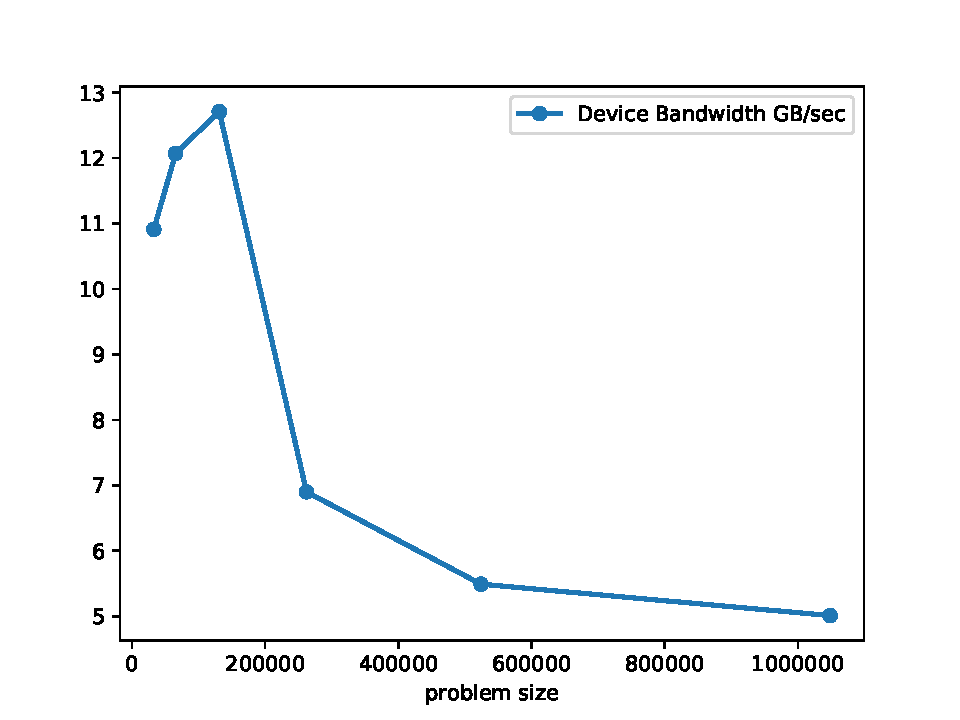
\includegraphics[scale=0.65]{graph.pdf}
\end{figure}

\subsection{}
For this problem, compared to problem 2, we are doing many more reads for each kernel call. The number of reads increases as the average edge size increases. This is reflected in the bandwidth measurements, where bandwidth decreases as average number of edges increases.

For example, with an average number of edges we are doing 31 reads and we get slightly more than 1/31 of the theoretical peak performance.

\tiny{\verbatiminput{../q2_results.txt}}


\end{document}